\documentclass{article}
\usepackage{graphicx}
\graphicspath{ {images/} }
%%%%%%%%%%%%%%%%%%%%%%%%%%%%%%%%%%%%%%%%%
% Lachaise Assignment
% Structure Specification File
% Version 1.0 (26/6/2018)
%
% This template originates from:
% http://www.LaTeXTemplates.com
%
% Authors:
% Marion Lachaise & François Févotte
% Vel (vel@LaTeXTemplates.com)
%
% License:
% CC BY-NC-SA 3.0 (http://creativecommons.org/licenses/by-nc-sa/3.0/)
% 
%%%%%%%%%%%%%%%%%%%%%%%%%%%%%%%%%%%%%%%%%

%----------------------------------------------------------------------------------------
%	PACKAGES AND OTHER DOCUMENT CONFIGURATIONS
%----------------------------------------------------------------------------------------



\usepackage{amsmath,amsfonts,stmaryrd,amssymb} % Math packages

\usepackage{enumerate} % Custom item numbers for enumerations

\usepackage[ruled]{algorithm2e} % Algorithms

\usepackage[framemethod=tikz]{mdframed} % Allows defining custom boxed/framed environments

\usepackage{listings} % File listings, with syntax highlighting
\lstset{
	basicstyle=\ttfamily, % Typeset listings in monospace font
}

%----------------------------------------------------------------------------------------
%	DOCUMENT MARGINS
%----------------------------------------------------------------------------------------

\usepackage{geometry} % Required for adjusting page dimensions and margins

\geometry{
	paper=a4paper, % Paper size, change to letterpaper for US letter size
	top=2.5cm, % Top margin
	bottom=3cm, % Bottom margin
	left=2.5cm, % Left margin
	right=2.5cm, % Right margin
	headheight=14pt, % Header height
	footskip=1.5cm, % Space from the bottom margin to the baseline of the footer
	headsep=1.2cm, % Space from the top margin to the baseline of the header
	%showframe, % Uncomment to show how the type block is set on the page
}

%----------------------------------------------------------------------------------------
%	FONTS
%----------------------------------------------------------------------------------------

\usepackage[utf8]{inputenc} % Required for inputting international characters
\usepackage[T1]{fontenc} % Output font encoding for international characters

% \usepackage{XCharter} % Use the XCharter fonts

%----------------------------------------------------------------------------------------
%	COMMAND LINE ENVIRONMENT
%----------------------------------------------------------------------------------------

% Usage:
% \begin{commandline}
%	\begin{verbatim}
%		$ ls
%		
%		Applications	Desktop	...
%	\end{verbatim}
% \end{commandline}

\mdfdefinestyle{commandline}{
	leftmargin=10pt,
	rightmargin=10pt,
	innerleftmargin=15pt,
	middlelinecolor=black!50!white,
	middlelinewidth=2pt,
	frametitlerule=false,
	backgroundcolor=black!5!white,
	frametitle={Command Line},
	frametitlefont={\normalfont\sffamily\color{white}\hspace{-1em}},
	frametitlebackgroundcolor=black!50!white,
	nobreak,
}

% Define a custom environment for command-line snapshots
\newenvironment{commandline}{
	\medskip
	\begin{mdframed}[style=commandline]
}{
	\end{mdframed}
	\medskip
}

%----------------------------------------------------------------------------------------
%	FILE CONTENTS ENVIRONMENT
%----------------------------------------------------------------------------------------

% Usage:
% \begin{file}[optional filename, defaults to "File"]
%	File contents, for example, with a listings environment
% \end{file}

\mdfdefinestyle{file}{
	innertopmargin=1.6\baselineskip,
	innerbottommargin=0.8\baselineskip,
	topline=false, bottomline=false,
	leftline=false, rightline=false,
	leftmargin=2cm,
	rightmargin=2cm,
	singleextra={%
		\draw[fill=black!10!white](P)++(0,-1.2em)rectangle(P-|O);
		\node[anchor=north west]
		at(P-|O){\ttfamily\mdfilename};
		%
		\def\l{3em}
		\draw(O-|P)++(-\l,0)--++(\l,\l)--(P)--(P-|O)--(O)--cycle;
		\draw(O-|P)++(-\l,0)--++(0,\l)--++(\l,0);
	},
	nobreak,
}

% Define a custom environment for file contents
\newenvironment{file}[1][File]{ % Set the default filename to "File"
	\medskip
	\newcommand{\mdfilename}{#1}
	\begin{mdframed}[style=file]
}{
	\end{mdframed}
	\medskip
}

%----------------------------------------------------------------------------------------
%	NUMBERED QUESTIONS ENVIRONMENT
%----------------------------------------------------------------------------------------

% Usage:
% \begin{question}[optional title]
%	Question contents
% \end{question}

\mdfdefinestyle{question}{
	innertopmargin=1.2\baselineskip,
	innerbottommargin=0.8\baselineskip,
	roundcorner=5pt,
	nobreak,
	singleextra={%
		\draw(P-|O)node[xshift=1em,anchor=west,fill=white,draw,rounded corners=5pt]{%
		Question \theQuestion\questionTitle};
	},
}

\newcounter{Question} % Stores the current question number that gets iterated with each new question

% Define a custom environment for numbered questions
\newenvironment{question}[1][\unskip]{
	\bigskip
	\stepcounter{Question}
	\newcommand{\questionTitle}{~#1}
	\begin{mdframed}[style=question]
}{
	\end{mdframed}
	\medskip
}

%----------------------------------------------------------------------------------------
%	WARNING TEXT ENVIRONMENT
%----------------------------------------------------------------------------------------

% Usage:
% \begin{warn}[optional title, defaults to "Warning:"]
%	Contents
% \end{warn}

\mdfdefinestyle{warning}{
	topline=false, bottomline=false,
	leftline=false, rightline=false,
	nobreak,
	singleextra={%
		\draw(P-|O)++(-0.5em,0)node(tmp1){};
		\draw(P-|O)++(0.5em,0)node(tmp2){};
		\fill[black,rotate around={45:(P-|O)}](tmp1)rectangle(tmp2);
		\node at(P-|O){\color{white}\scriptsize\bf !};
		\draw[very thick](P-|O)++(0,-1em)--(O);%--(O-|P);
	}
}

% Define a custom environment for warning text
\newenvironment{warn}[1][Warning:]{ % Set the default warning to "Warning:"
	\medskip
	\begin{mdframed}[style=warning]
		\noindent{\textbf{#1}}
}{
	\end{mdframed}
}

%----------------------------------------------------------------------------------------
%	INFORMATION ENVIRONMENT
%----------------------------------------------------------------------------------------

% Usage:
% \begin{info}[optional title, defaults to "Info:"]
% 	contents
% 	\end{info}

\mdfdefinestyle{info}{%
	topline=false, bottomline=false,
	leftline=false, rightline=false,
	nobreak,
	singleextra={%
		\fill[black](P-|O)circle[radius=0.4em];
		\node at(P-|O){\color{white}\scriptsize\bf i};
		\draw[very thick](P-|O)++(0,-0.8em)--(O);%--(O-|P);
	}
}

% Define a custom environment for information
\newenvironment{info}[1][Info:]{ % Set the default title to "Info:"
	\medskip
	\begin{mdframed}[style=info]
		\noindent{\textbf{#1}}
}{
	\end{mdframed}
}
 % Include the file specifying the document structure and custom commands
\def\code#1{\texttt{#1}}
% \newcommand{\code}[1]{\colorbox{light-gray}{\texttt{#1}}}
										%-------------------------------%
										%	ASSIGNMENT INFORMATION		%
										%-------------------------------%

\title{LIS4031: Project \#3} % Title of the assignment

\author{Jose Carlos Archundia Adriano - Carlos Andres Reyes Evangelista - Erick Siordia Nagaya\\ \texttt{jose.archundiaao@udlap.mx - carlos.reyesea@udlap.mx - erick.siordiana@udlap.mx}} % Authors name and email addresses

\date{Universidad de las Am\'ericas  Puebla --- \today} % University, school and/or department name(s) and a date

										%-------------------------------%
										%			DOCUMENT			%
										%-------------------------------%

\begin{document}

\maketitle % Print the title

%-------------------------------%
%		INTRODUCTION			%
%-------------------------------%
\section{Abstract}
The Vector Space Model is a retrieval model used to search and rank data in a collection of documents. The implementation of this model is useful in the Information Retrieval area, as it allows for the retrieval of documents in a collection that are relevant to a specific query. Based on the Vector Space Model, an implementation was developed using the Cranfield Collection as the test collection. In order to quantify the quality of the retrieved documents, the precision and recall of documents were used as metrics and calculated by averaging random queries results.
The implementation of the Vector Space retrieval model performs its search on articles provided by the Cranfield Collection, and compares the results to the suggested relevant documents included in the collection. It is also able to calculate the precision and recall of 10 random queries, and show the results as a graph..


\section{Introduction}
The Vector Space Model is an information retrieval model described as a «simple and intuitively appealing framework for implementing term weighting, ranking and relevance feedback» by Bruce Croft et al. (2015). It works by «assuming that documents and queries are part of a \textit{t}-dimensional vector space, where \textit{t} is the number of index terms» according to Bruce Croft et al. (2015). Each of these terms is weighed according to the formula:
\begin{equation}
	idf_{t}=\log_{10}(\frac{N}{df_{t}})
\end{equation}
Where $N$ is the total number of documents and $df_{t}$ represents the total number of documents where $_{t}$ appears. After these \textit{global} weights are computed, they are multiplied by the frequency with which each term appears in the document they are in to finish the creation of the document's vector representation. The scalar product between each document vector and the query vector is obtained to get a \textit{similarity coefficient} for each document. Finally, the documents are sorted according to its \textit{similarity coefficient}, the document with the highest \textit{similarity coefficient} being the most relevant document.



\section{Objective}
This project aims to achieve a fully-functional implementation of the Vector Space Model for information retrieval. The delivered software must be able to parse an already proven test collection, and let the user choose among a set of preprocessed queries in order to compute and display the most relevant results for that given query. These results must be rendered based on their relevance to the query. As an extra feature, the software must provide an option to select 10 random queries, compute their precision and recall, and graph its average.

\section{Description of the problem}
When storing large quantities of data in collections, it is useful to have a system able to swiftly find useful information that a user is requesting. In order to do this, an algorithm is needed to determine the relevance of each article or document in the collection based on the needs of the user. As explained before, the Vector Space retrieval model allows the assignment of a weight to each document of the collection based on the frequency of the terms it contains. For this software, the Cranfield Collection will be used as the collection of documents, and the developed algorithm will have to analyze each document and their terms in order to compute their relevance coefficient relative to a user-selected query. Through this process, a relevance-sorted list of documents can be returned to the user.
To evaluate this retrieval system, precision and recall are used to quantify the quality of the retrieved data.


\section{Methodology}
The implementation of this project was developed with the programming language \textbf{Kotlin}: a multi-paradigm language with a focus on object-oriented and functional programming. This decision was taken due to the tight coupling of back-end and front-end programming with the framework \textbf{TornadoFX}.

The project is structured under a Model-View-Controller architecture with classes as follows:

\begin{itemize}
	\item \textbf{View} {
		\begin{itemize}
			\item \textbf{Home} {
				This view represents the first screen the user is presented with. A screenshot is presented in \textit{Figure 3}.
			}
			\item \textbf{Results} {
				This view shows the same controls as the first one, but also displays the list of results of the selected query. It can be seen in \textit{Figure 4}.
			}
			\item \textbf{Chart} {
				Finally, in this view is a rendered chart containing the average metrics among 10 random queries. It is shown in \textit{Figure 5}
			}
		\end{itemize}
	}

	\item \textbf{Controller} {
		This \textit{controller} works as a middleman among the \textit{view} and \textit{model} classes. It handles user inputs and performs the corresponding task in the \textit{model} and updates the \textit{view} based on changes in the \textit{model} .
	}


	\item \textbf{Model} {
		\begin{itemize}
			\item \textbf{Reader} {
				This backend module provides an API to load articles, queries, and relevant from the disk into memory. It also performs some pre-analysis tasks to organize the data for further usage. The IDF for each term is calculated here.
			}
			\item \textbf{VectorSpaceModel} {
				This class implements the actual functionality of a Vector Space retrieval model. Using the data structures provided by \code{Reader}, it generates the document and query weighted vectors -with the previously defined formula-, and computes the similarity coefficient between them. By using these results, it also creates the ranked results list for a given query. Finally, it performs the required actions to choose the random queries and return their precision and recall averages.
			}
		\end{itemize}
	}
\end{itemize}

The algorithm for the main functionality of the document search based on a given query is illustrated in \textit{Figure 4}.

On startup, the Reader class is in charge of parsing the \textit{Cranfield Collection} and generating object to represent the queries, articles, and relevance lists in memory. The Reader also tokenizes the terms in both the queries and the articles, and saves them internally for use later. From these token sets, the IDF of each token is calculated. The diagram illustrated in the \textit{Figure 1} demonstrates the process of searching a given query. First, the Home View calls the Controller on startup. The Controller asks the VSM for the list of queries to display. This is provided by fetching the list from the Reader, and relaying it all the way back to Home. Home is then rendered and waits for user input. After detecting the user's intention to search a selected query, it send the query to the VSM by relaying it through the controller. The VSM fetched additional data from Reader, and calculates the similarity coefficients of each article with respect to the selected query. The list of articles is sorted based on this coefficient, and relayed back to the controller. The controller then switches the view to the Results view, which displays the ranked article list. This similarity coefficient is computed with the function shown in the \textit{Figure 6}. This value is computed as the sum of the product of each term weight and its frequency in the article, and the weight of the term in the query; as shown in the last line of the for loop of the function. A more detailed execution of this function is show in the \textit{Figure 7}, where the query vector can be observed with its terms and weights, along with the document data: content, id and title.

On other hand, the diagram illustrated in the \textit{Figure 2} shows the process of generating 10 random query results and calculating the average precision and recall. First, the user signals the Home view by pressing the precision/recall button. The Home view then informs the controller of this action, causing the controller to switch the view to the Chart view which will show the final results, and asks the VSM for the precision and recall of 10 random queries. The VSM selects 10 random queries and fetches query and article info from the Reader. The VSM then searches for 10 ranked article lists corresponding to the random queries. The precision and recall are calculated based on these lists and returned to the controller as a pair, which is then handed to the Chart view to render as a graph.




\section{Results and analysis}
When the implementation of the system was done, the results of the test queries where analyzed based on the \textit{cranrel} file to know if the ranking assigned to the files is similar to the one specified in the relevance evaluation test file.

As seen in \textit{Figure 4}, the top results returned for the query with ID 1 are the documents with IDs 1286, 13, 184, 14, and 51. In this case, the ID 1286 is not found in \textit{cranrel}, but the other articles are present in the \textit{cranrel} file, and are marked as relevant to some degree for that query. The relevance coefficient for these queries may vary in the \textit{cranrel} file, however, we can observe that there exists an overlap between these two sets of results.

For the evaluation of the model, the obtained results performed as expected due to the behavior of the data. As we can see in the \textit{Figure 5}, the average recall increases over time because the model finds more relevant articles over time, although the precision also decreases because of the non-relevant articles that were found by the search engine.
It is also important to note that the values obtained in the average metrics are very low due to the fact that each query only has, on averge, 10 to 20 relevant documents. Because of this ratio of relevant documents to total number of documents, the obtained precission and recall will always be extremely low.


\section{Conclusion}
In the development of this project, different challenges were faced. Specially, the development of the Graphical User Interface was considered to be the biggest challenge. This is because it was necessary to build a responsive UI that adapted to user input. The reason behind the difficulty of this task was the refined management for each action performed in the program. To manage the events and actions, language specific features like properties and observables were used to deal with the asynchronous tasks and communications between the front-end and the back-end.
Other challenges were faced, like the parsing of the articles and queries of the test collection and the implementation of the Vector Space Model. However, the team considered that the biggest factors in the difficulty of those tasks were due to the use of a \textit{Kotlin}, a programming language that was new for some team members, and the use of tools like IntelliJ IDE, which required a small learning curve for some features.

From the results generated by our random precision and recall graph, we can see that the Vector Space Model does, on average, produce relevant documents to a given query. However, this is only true for the first few documents the Vector Space Model produces. This is due to the fact that the Vector Space retrieval model compares the \textit{frequency} of terms, and does not perform any kind of linguistic processing or classification techniques. Additional steps can be taken to improve the results of the Vector Space retrieval model, such as using stemming or lemmatization. By applying linguistic processing techniques before ranking documents, we can improve both the precision and recall of our retrieval system.

Our team was able to successfully overcome these challenges and develop a working application which implemented the Vector Space Model for the retrieval of documents relevant to a given query. We were able to further our understanding of retrieval systems as well as exercise our programming skills in a project that allowed us to demonstrate the concepts that we have learned in class.



\section{References}
Croft, B., Metzler, D. and Strohman, T. (2015). \textit{Search engines: Information Retrieval in Practice}. 2nd ed. Pearson Education, Inc.


\section{Appendix}

\begin{figure}[h]
	\caption{Sequence diagram for searching a query}
	\centering
	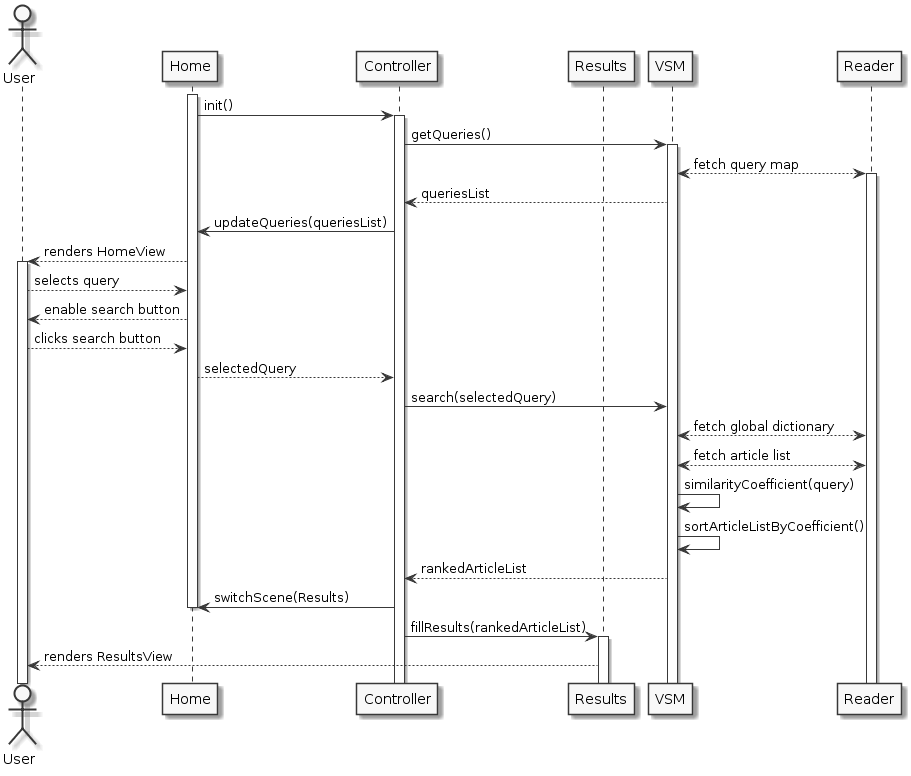
\includegraphics[scale=0.5]{searchDiagram}
\end{figure}

\begin{figure}[h]
	\caption{Sequence diagram for generating precision and recall random data}
	\centering
	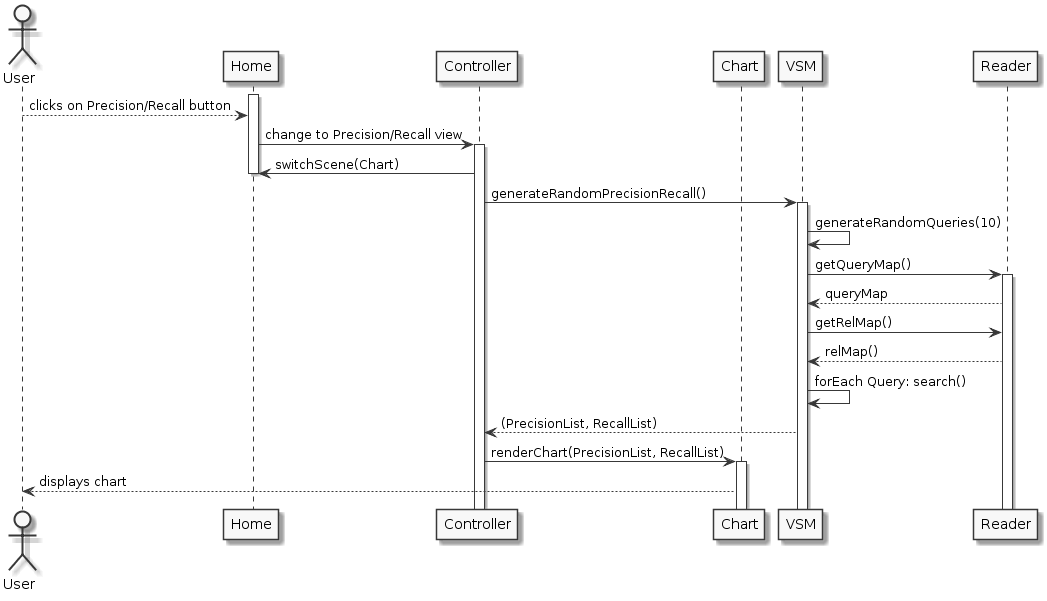
\includegraphics[scale=0.4]{precisionRecallDiagram}
\end{figure}

\begin{figure}[h]
	\caption{Home View}
	\centering
	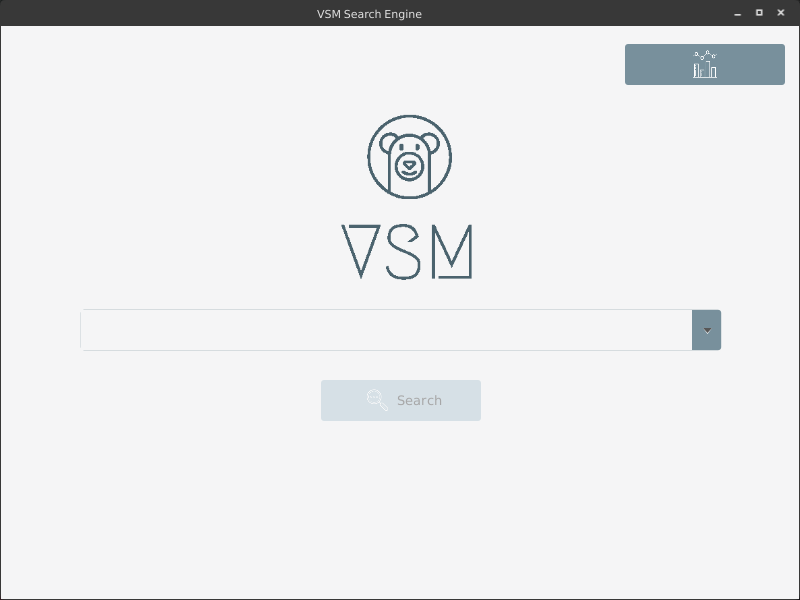
\includegraphics[scale=0.5]{home}
\end{figure}

\begin{figure}[h]
	\caption{Results for query 1.}
	\centering
	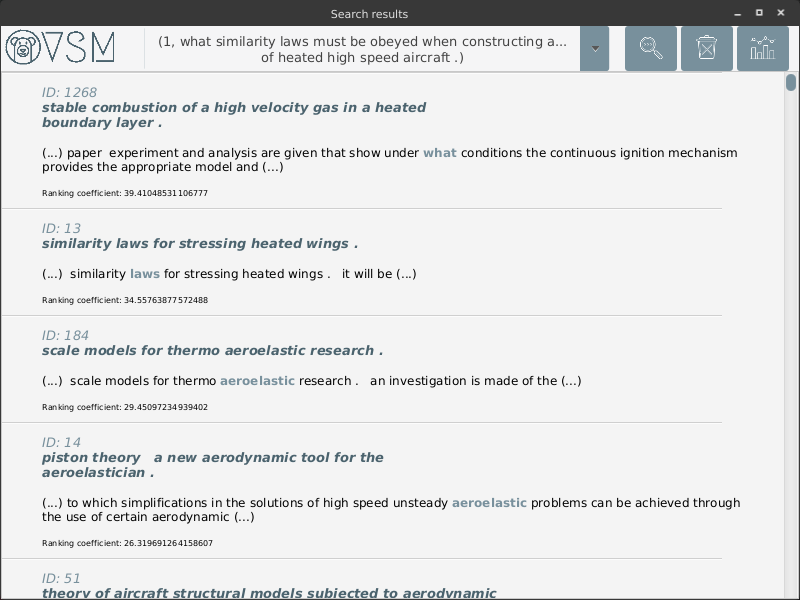
\includegraphics[scale=0.5]{query1Results}
\end{figure}

\begin{figure}[h]
	\caption{Evaluation chart for the retrieval model}
	\centering
	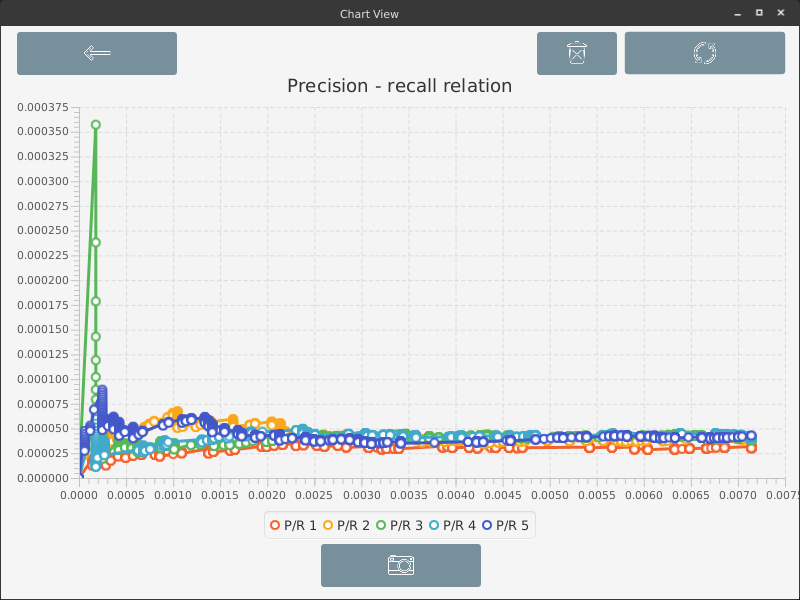
\includegraphics[scale=0.5]{modelEvaluation}
\end{figure}

\begin{figure}[h]
	\caption{getSimilarityCoefficent function}
	\centering
	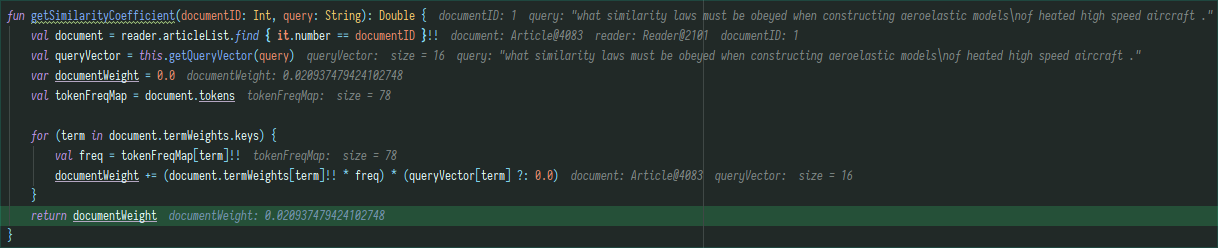
\includegraphics[scale=0.4]{documentWeightsFunction}
\end{figure}

\begin{figure}[h]
	\caption{getSimilarityCoefficent function variables under execution}
	\centering
	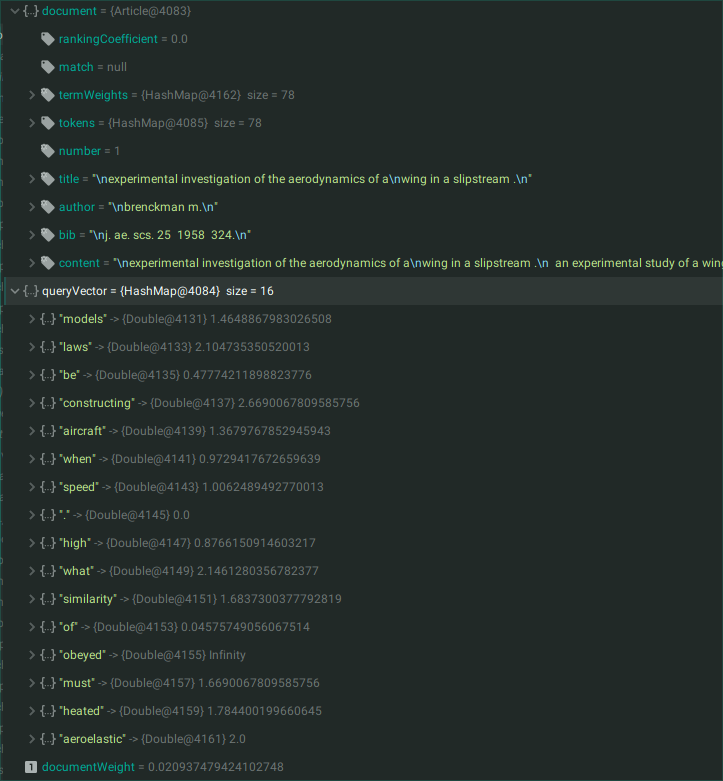
\includegraphics[scale=0.4]{documentWeights}
\end{figure}

%----------------------------------------------------------------------------------------
\end{document}
